
\documentclass[tikz, border=10pt]{standalone}
\usepackage{tikz}
\usetikzlibrary{positioning, chains, shapes.geometric, fit, shapes, arrows.meta, calc, backgrounds}

\begin{document}
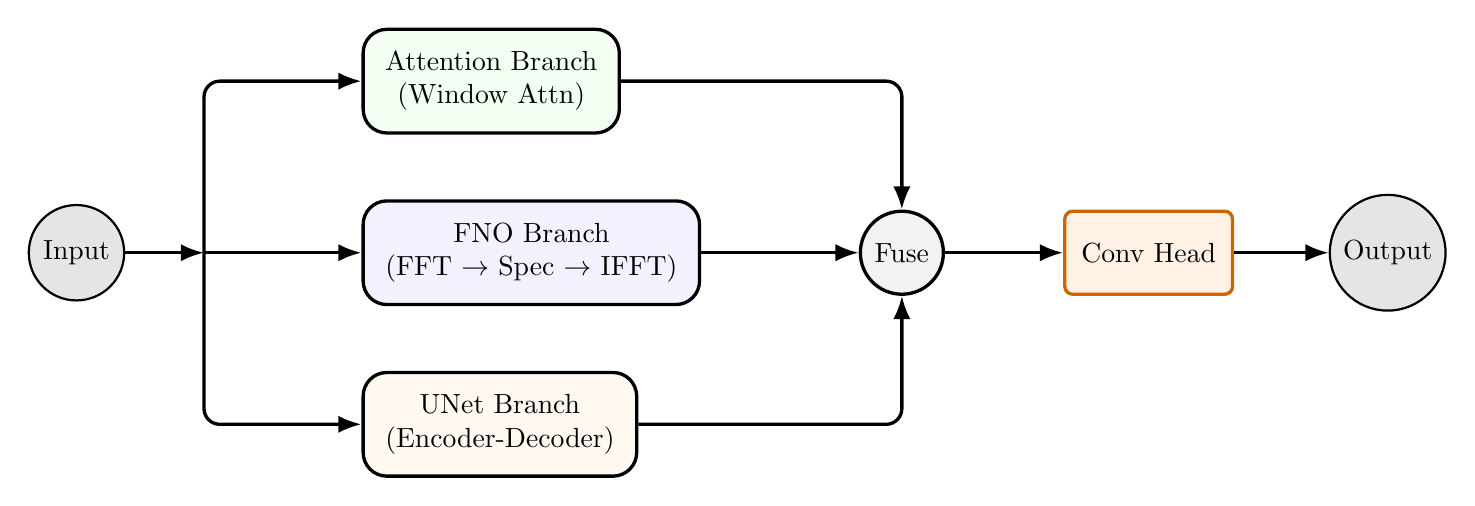
\begin{tikzpicture}[
    >=LaTeX, 
    very thick,
    node distance=1.0cm and 1.2cm,
    arrow/.style={
        ->,
        very thick,
        rounded corners=0.2cm
    },
    block/.style={
        rectangle,
        fill=gray!10,
        rounded corners=3mm,
        draw,
        very thick,
        inner sep=0.8em
    },
    layer/.style={
        rectangle,
        fill=white!10,
        rounded corners=1mm,
        inner xsep=0.6em,
        inner ysep=0.6em,
        minimum height=3.0em,
        align=center,
        draw,
        very thick
    },
    conv/.style={
        layer,
        fill=orange!10,
        draw=orange!80!black
    },
    relu/.style={
        layer,
        fill=yellow!10,
        draw=yellow!80!black,
        minimum height=2.5em
    },
    pool/.style={
        layer,
        fill=red!10,
        draw=red!80!black
    },
    input/.style={ 
        circle,
        minimum width=3.0em,
        draw,
        fill=gray!20,
        thick,
        align=center
    },
    sum/.style={
        circle,
        draw,
        fill=white,
        inner sep=0pt,
        minimum size=1.2em,
        node contents={+}
    }
]


    \node[input] (in) {Input};
    
    % Split point
    \coordinate[right=1.0cm of in] (split);
    \draw[arrow] (in) -- (split);

    % --- Top Branch: Attention ---
    \node[block, above right=1.5cm and 2.0cm of split, fill=green!5, align=center] (attn_branch) {Attention Branch\\(Window Attn)};
    \draw[arrow] (split) |- (attn_branch.west);

    % --- Middle Branch: FNO ---
    \node[block, right=2.0cm of split, fill=blue!5, align=center] (fno_branch) {FNO Branch\\(FFT $\to$ Spec $\to$ IFFT)};
    \draw[arrow] (split) -- (fno_branch.west);

    % --- Bottom Branch: UNet ---
    \node[block, below right=1.5cm and 2.0cm of split, fill=orange!5, align=center] (unet_branch) {UNet Branch\\(Encoder-Decoder)};
    \draw[arrow] (split) |- (unet_branch.west);

    % --- Fusion ---
    \node[circle, draw, right=2.0cm of fno_branch, minimum size=3em, fill=gray!10] (fusion) {Fuse};
    
    \draw[arrow] (attn_branch.east) -| (fusion.north);
    \draw[arrow] (fno_branch.east) -- (fusion.west);
    \draw[arrow] (unet_branch.east) -| (fusion.south);

    % Head
    \node[conv, right=1.5cm of fusion] (head) {Conv Head};
    \node[input, right=of head] (out) {Output};

    \draw[arrow] (fusion) -- (head);
    \draw[arrow] (head) -- (out);

\end{tikzpicture}
\end{document}
